% v 1.9
\section{Experimental Setup}
%
\label{sec:expsetup}

As illustrated in Fig.~\ref{pic:expsetup}, this experiment will study electron scattering from a 15 cm long 
liquid Deuterium target held in a vacuum.
The scattered electron will be detected in the BigBite spectrometer with an upgraded electron detector stack. 
The neutron arm is arranged with a dipole magnet 48D48 (SBS) and a segmented hadron calorimeter HCAL.  
The whole detector package was designed and is now under assembling for the GMn, E12-09-019, experiment. 

\begin{figure}[bh]
	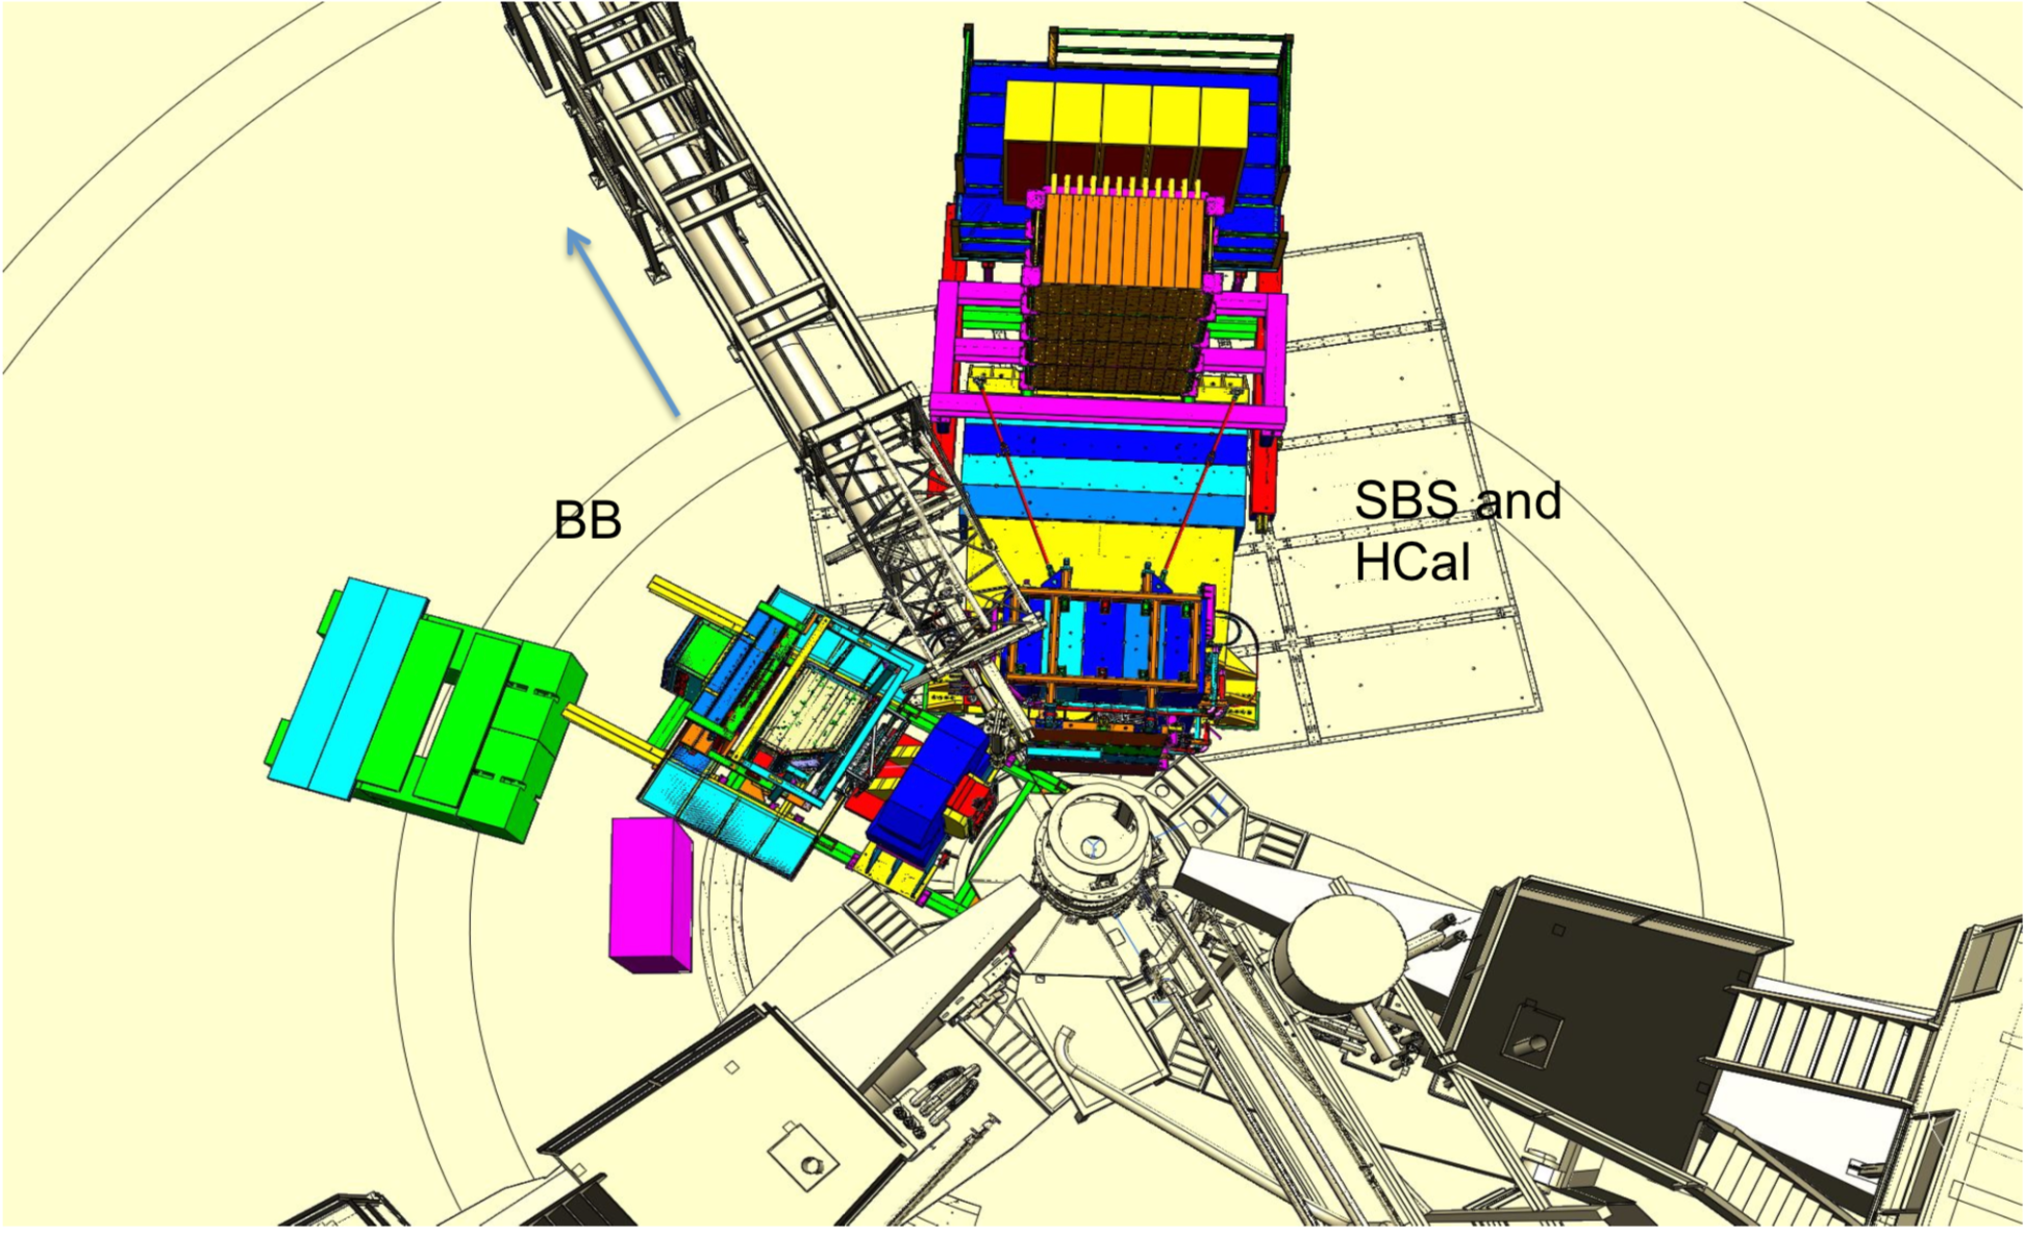
\epsfig{file=Plots/Exp_setup_3D.pdf, height=3.0in}
	\caption{Layout of the experimental setup in nTPE.}	
\label{pic:expsetup}
\end{figure}

\subsubsection{Parameters of the SBS}

The 48D48 magnet from Brookhaven was acquired as part of the Super Bigbite project and will be available for this experiment.  
It consists of a large dipole magnet which provides a field integral of about 1.7~ T $\cdot$ m, allowing for quasielastic 
protons to be sufficiently deflected to allow clear differentiation from neutrons.  
The active field volume has an opening of $46 \times$ 25 vertical $\times$ horizontal), 
matching the aspect ratio of the neutron arm, and a depth of 48 cm.

The placement of this magnet will be 1.6 m away from the target, which would normally interfere with the beamline.  
To accommodate this, modifications were made to the iron yoke such that the beamline will pass through the magnet yoke area.

The field configuration will be such that positively charged particles will be deflected upwards away from the hall floor.  
For a field integral of 1.7 Tesla-m, protons of momentum 2.5 GeV/c will be deflected 250 mrad,
 which translates to a displacement of xxm.  
 Including expected detector resolution,  the $p_{miss,\perp}$ distribution will be similar to 
 what was seen in E02-013, so cuts of  $< 100$ MeV/c will be appropriate.  
Monte Carlo simulations show a contamination of charged quasielastics to be negligible.

The presence of the magnet also works to sweep low energy charged particles from the target away from the neutron arm.  
Particles of momentum less than 1.3~{GeV/c} will be entirely swept outside of the neutron arm acceptance.  
This greatly reduces the amount of charged low energy background.
%

